\documentclass[11pt]{beamer}
\usepackage{graphicx}

\usepackage{amsmath}
\usepackage{amssymb}

\usepackage{xcolor}
\usepackage{biblatex}

\usepackage{bbding}

\usepackage[noend]{algpseudocode}
\usepackage{algorithm}
\makeatletter
\renewcommand{\ALG@beginalgorithmic}{\small}
\makeatother

\bibliography{01_indexing_intro}
\bibliography{02_fingerprint_indexing}
\bibliography{03_vector_database}

\usetheme{Madrid}
\setbeamertemplate{navigation symbols}{}

\renewcommand{\footfullcite}[1]{%
  \footnote{\scriptsize \citeauthor{#1}, {\color{beamer@blendedblue} \citetitle{#1}}, \citeyear{#1}}%
}

\title{Apresentação: HNSW}
\author{João Felipe}
\date{}



\begin{document}

\begin{frame}
\vspace{1.8em}
\maketitle
\vspace{-4em}
\begin{center}
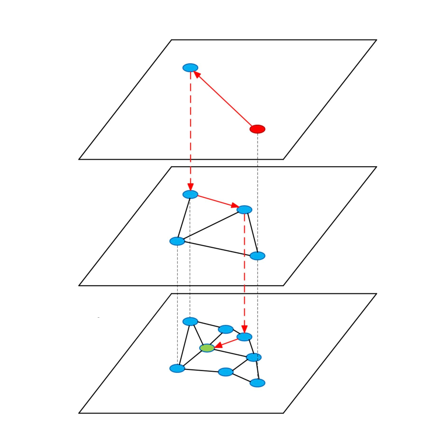
\includegraphics[width=.35\textwidth]{imgs/hnsw_min.png}
\end{center}
\end{frame}

\begin{frame}{Definição do Problema}


\textbf{Indexação}:

\begin{enumerate}
    \item \textbf{Representação}: Representar os dados de uma maneira que seja possível avaliar a semelhança entre eles. \footfullcite{surveyfeatures:schuch2019}\footfullcite{surveyfpindex:gupta2019} 
    
    \HandRight Foco dos estudos de fingerprint.
    \item \textbf{Estrutura de dados}: Construir o índice.
\end{enumerate}

\begin{figure}
    \centering
    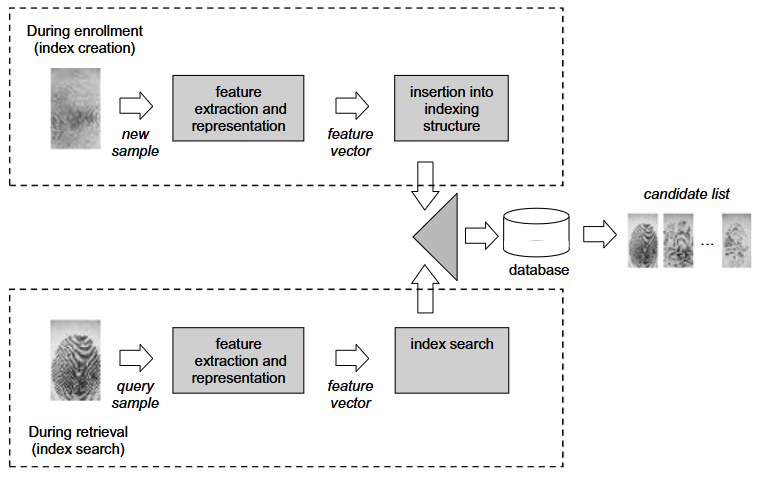
\includegraphics[width=0.45\linewidth]{imgs/indexing_fp.png}
    \vspace{-1em}
    \caption{\scriptsize Esquema de indexação \footfullcite{bookfingerrec:maltoni2009}}
\end{figure}

\end{frame}

\begin{frame}{Exemplos}
    Exemplos de indexação baseada em minúcias.

    \begin{figure}
        \centering
        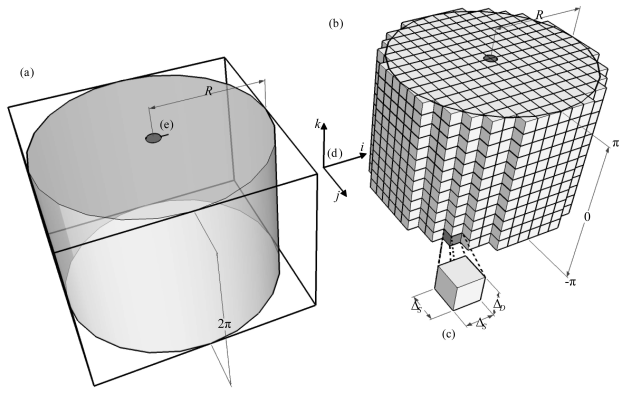
\includegraphics[width=0.45\linewidth]{imgs/fingerprint_cylinder_code.png}
        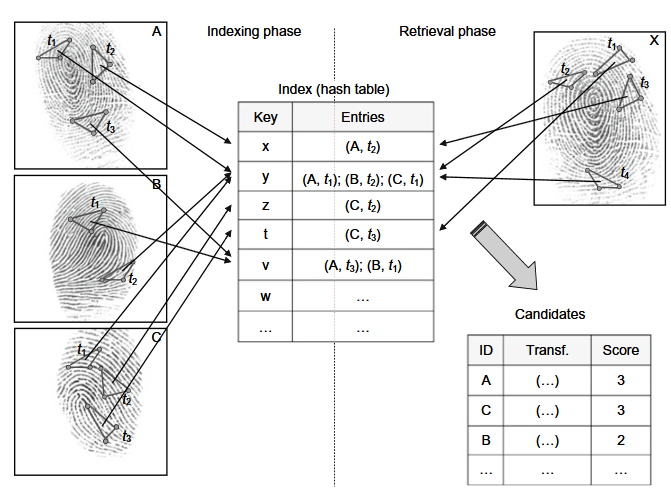
\includegraphics[width=0.45\linewidth]{imgs/minutia_triplets.png}
        \caption{\scriptsize Primeiro exemplo: Minutia Cylinder-Code (MCC) + Locality-Sensitive Hashing (LSH). Segundo exemplo: Minutia Triplets + Hash Table}
    \end{figure}
\end{frame}

\begin{frame}{Exemplos}
\begin{figure}
    \centering
    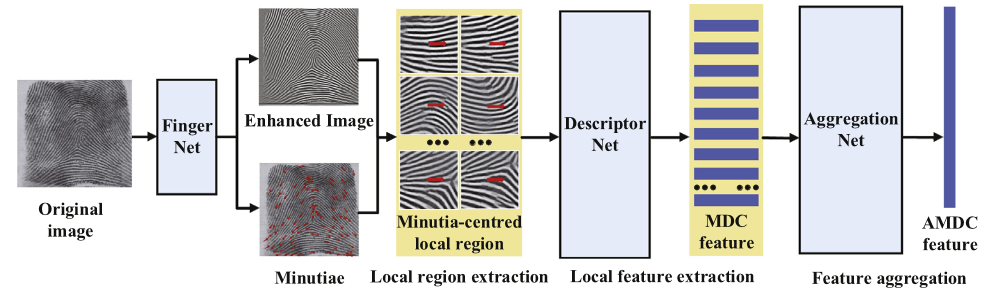
\includegraphics[width=0.9\linewidth]{imgs/aggregating_mdc.png}
    \caption{\scriptsize AMDC: Aggregated Minutia-centred Deep Convolutional + Scan linear, i.e., distância entre query e toda a galeria.}
\end{figure}
\end{frame}

\begin{frame}{Soluções}

É mais interessante contar com uma estrutura otimizada para...

\begin{itemize}
    \item Busca dos k vizinhos mais próximos (k-NNS)
    \item Existem estruturas acelerar k-NNS exata.\footfullcite{multidimensionalmethods:gaede1998}\footfullcite{searching:chavez2001}\footfullcite{surveyexactknn:ukey2023} 
    
    *Escalabilidade ruim com relação a \textit{dimensionalidade intrínseca} dos dados.
\end{itemize}

\end{frame}

\begin{frame}{Maldição da dimensionalidade}

``Curse of dimensionality":
\begin{itemize}
    \item A complexidade desses métodos para dimensões altas é linear. Experimento mostram que a força bruta é mais rápida.\footfullcite{quantitative:weber1998}
    \item A distância até o vizinho mais próximo tende a distância até o vizinho mais distante \footfullcite{meaningful:beyer1999}
    \item Alguns outros fatos: a razão de volumes entre um cubo e uma esfera inscrita em seu interior vai a zero, quando as dimensões crescem (existe muito espaço vazio); a média da distribuição de distância aumenta, enquanto que a variância colapsa (quase todos pontos tem mesma distância entre si) \footfullcite{effects:kouiroukidis2011}.
\end{itemize}

\end{frame}

\begin{frame}{Maldição da dimensionalidade}
    \begin{figure}
        \centering
        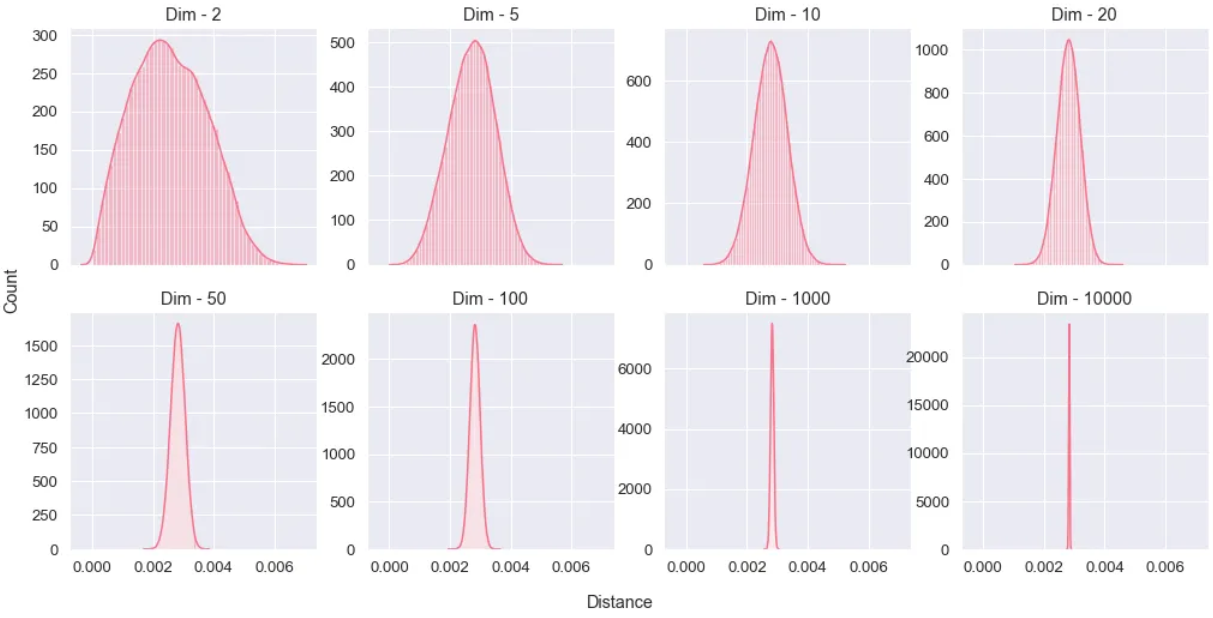
\includegraphics[width=0.85\linewidth]{imgs/curse_of_dim.png}
        \caption{\scriptsize Distância entre pares de pontos gerados uniformemente.}
    \end{figure}
\end{frame}

\begin{frame}{Approximate Nearest Neighbor Search (ANNS)}
\begin{itemize}
    \item Relaxar a condição do problema. Retornar os $k$ mais próximos, com uma taxa de acerto inferior a 100\%, chamada de \textit{recall}. Métodos ANNS.
\footfullcite{ann:aumuller2017}
\footfullcite{approximate:tian2023}
\footfullcite{comprehensive:han2023}
\footfullcite{survey:pan2024}
\end{itemize}

\begin{figure}
    \centering
    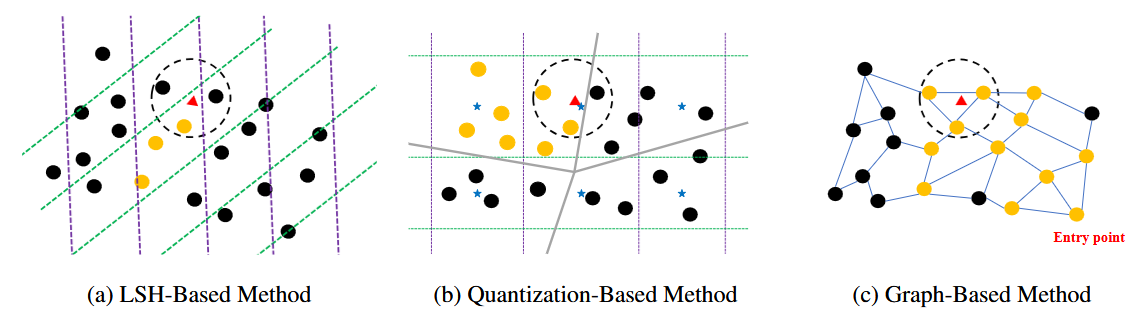
\includegraphics[width=0.8\linewidth]{imgs/approximate_methods.png}
\end{figure}
\end{frame}

\begin{frame}{Hierarchical Navigable Small World (HNSW)}
    O ``campeão" dos benchmarks.

    \begin{figure}
        \centering
        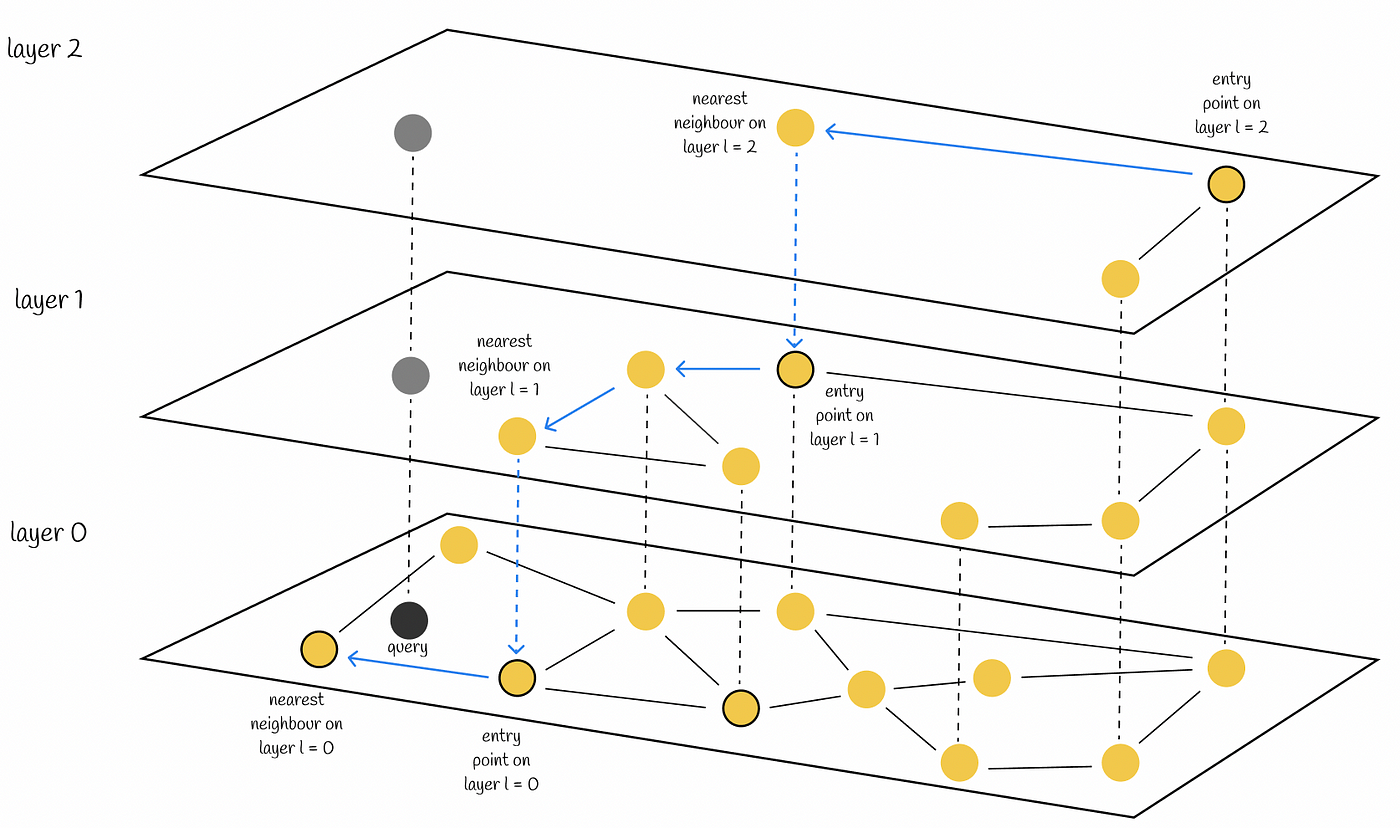
\includegraphics[width=0.4\linewidth]{imgs/hnsw_search.png}
        \caption{Ilustração da busca em HNSW.}
    \end{figure}

    {\scriptsize Funciona buscando por camadas, começando da primeira, com menos elementos e links mais longos. Em cada camada, busca o elemento mais próximo e pula para a camada inferior.
    
    \textsc{Analogia} Ao invés de descrever uma viagem: R. Dr. Francisco de Toledo (BG-Campinas) $\to$ Roxo Moreira (BG-Campinas) $\to$ ... $\to$ D. Pedro $\to$ ... $\to$ Av. Norte Sul (Brag. Pta.) $\to$ R. Itaparica (Brag. Pta.). Prefiro, descrever do macro para o micro.}
\end{frame}

\begin{frame}{SA Tree}

Para entender o método, começamos com a Spatial Approximation Tree (SA Tree) \footfullcite{searching:gonzalonavarro2002}.

\begin{itemize}
    \item O nome vem da estratégia de se aproximar iterativamente do elemento mais próximo de forma gulosa, até alcançar o mínimo global.

    * Diferença comparado aos métodos de divisão espacial.
    \item Como garantir o mínimo global?
    \item Grafo completo satisfaz, mas seria inviável...
\end{itemize}
\end{frame}

\begin{frame}{SA Tree}
    \begin{itemize}
    
        \item O grafo com essas características recebe o nome de grafo de Delaunay (DG).
        \item Vizinhos de Voronoi são conectados.
        \begin{figure}
            \centering
            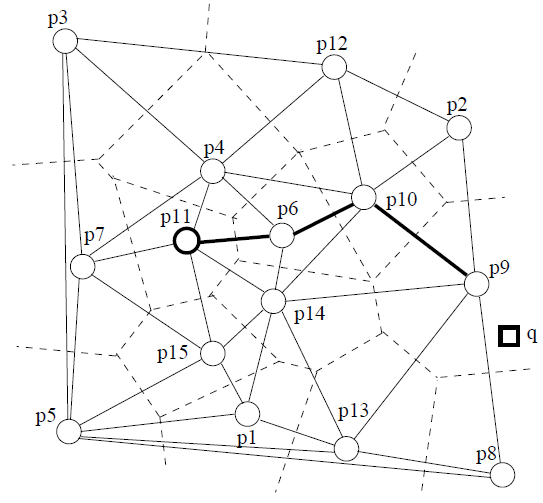
\includegraphics[width=0.3\linewidth]{imgs/delaunaysearch.png}
            \caption{\scriptsize Linhas sólidas são arestas do grafo, linhas pontilhadas são regiões de Voronoi, vértices são os elementos.}
        \end{figure}
        
    \end{itemize}
\end{frame}

\begin{frame}{SA Tree}

    Problemas:

    \begin{itemize}

        \item Não é possível construir esse grafo conhecendo somente as distâncias entre eles.

        \item O grau dos vértices em um grafo de Delaunay cresce exponencialmente com a dimensão \footfullcite{voronoi:dwyer1993}.
        
    \end{itemize}
\end{frame}

\begin{frame}{Aproximações Delaunay}

\begin{itemize}
    \item O objetivo deveria ser então construir uma aproximação, ou um subgrafo, do DG.
    \item Alternativas seriam: Grafo de k vizinhos mais próximos (k-NNG) ou um grafo de vizinhança relativa (RNG).
    \item Heurística usada para RGN e no HNSW:

    {\small
        \begin{block}{Relative Neighbor Heuristic}
            Um elemento $x$ só será vizinho de um elemento $a$ se, e somente se, $d(x, a) < d(x, y)$ para todo $y$ vizinho de $x$.
        \end{block}
    }
    \item No entanto, todas essas técnicas apresentam escalabilidade de busca como lei de potência.

    * Considere começar a busca de um ponto distante.
\end{itemize}

\end{frame}

\begin{frame}{Navigable Small World (NSW)}

\begin{itemize}
    \item Criando links de longo alcance, os grafos deixam de ser subgrafos do DG, mas ganham o status de serem \textbf{navegáveis}, i.e., grafos com escalabilidade logarítmica ou polilogarítmica no número de hops durante a busca gulosa.
    \item Nesse contexto, surgem as técnicas baseadas em grafos Navigable Small World (NSW)\footfullcite{smallworldgraphs:malkov2014}.
    \begin{figure}
        \centering
        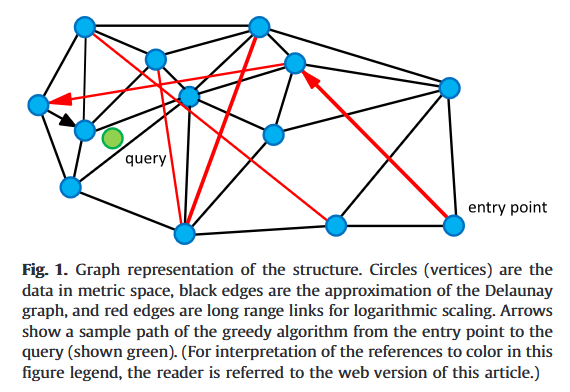
\includegraphics[width=0.5\linewidth]{imgs/navigablesmallworld_graph.png}
        \caption{\scriptsize Graph representation of the structure. Circles (vertices) are data in metric space, black edges are the approximation of the Delaunay graph, and red edges are long range links for logarithmic scaling. Arrows show a sample path of the greedy algorithm from the entry point to the query (shown green).}
        \label{fig:enter-label}
    \end{figure}
\end{itemize}

\end{frame}

\begin{frame}{NSW - k Nearest Search}

\begin{algorithm}[H]
\caption{NSW k Nearest Neighbors Search}\label{alg:NSW-KNNS}
\begin{algorithmic}[1]

\Procedure{NSW-kNNS}{object: $q$, int: $m$, int: $k$}
\State \text{tempRes}, \text{candidates}, \text{visited}, \text{result} $\gets$ new TreeSet
\For{$i \in 1..m$}
    \State Add random entry point to \text{candidates}
    \State $\text{tempRes} \gets \emptyset$
    \While{\textbf{true}}
        \State $c \gets \arg\min_{e \in \text{candidates}} d(e, q)$
        \State Remove $c$ from \text{candidates}
        \If{$d(c, q) \geq d(\text{result}[k], q)$} 
            \State \textbf{break}
        \EndIf
        \For{$e \in c.\text{friends}()$} 
            \If{$e \notin \text{visited}$}
                \State Add $e$ to \text{visited}, \text{candidates}, \text{tempRes}
            \EndIf
        \EndFor
    \EndWhile
    \State Merge \text{tempRes} into \text{result} 
\EndFor
\State \Return top $k$ elements from \text{result}
\EndProcedure
\end{algorithmic}
\end{algorithm}


\end{frame}

\begin{frame}{NSW - Build}

\begin{algorithm}[H]
\caption{NSW Build}\label{alg:NSWBuild}
\begin{algorithmic}[1]
\Procedure{NSW-Build}{object: new\_object, int: $f$, int: $w$}
\State neighbors $\gets$ \Call{NSW-kNNS}{new\_object, $w$, $f$}
\State \Call{BidirectLink}{$\text{neighbors}, \text{new\_object}$}
\EndProcedure
\end{algorithmic}
\end{algorithm}

\begin{itemize}
    \item O grafo pode ser facilmente construído de forma paralela, devido a natureza incremental e local de cada inserção.
    \item Considerando dados chegando em ordem aleatória, a propriedade de navigabilidade é emergente. Os links longos são aqueles mais antigos.
\end{itemize}

\end{frame}

\begin{frame}{NSW - Limitations}
    \begin{itemize}
        \item Escalabilidade polilogarítmica no número de cálculos de distância
        \begin{enumerate}
            \item $\text{(\# hops)}\sim O(\log n)$
                \item $\text{(degree of hubs)}\sim O(\log n)$
            \item $\text{(\# dist. computations) = (\# hops)(degree of hubs)} \sim O(\log^2 n)$
        \end{enumerate}
        \item Isso faz com que o método seja pior que algumas abordagens de árvore, que escalam com $\log n$, em determinados cenários.
        \item Como resolver esse problema? Parece que o item 2 pode ser atacado...
    \end{itemize}
\end{frame}

\begin{frame}{Hierarchical Navigable Small World (HNSW)}

\begin{quote}
    \small
    ``The idea of Hierarchical NSW algorithm is to separate the links according to their length into different layers and then search the multilayer graph. {\color{beamer@blendedblue}In this case, we can evaluate only a fixed number of the connections for each element independently of the network size, thus allowing logarithmic scalability}."\footfullcite{hnsw:malkov2018}
\end{quote}

\end{frame}

\begin{frame}{HNSW - Search Layer}

\begin{algorithm}[H]
\caption{HNSW Search Layer}\label{alg:HNSW-SL}
\begin{algorithmic}[1]
\Procedure{Search-Layer}{obj: $q$, list[obj]: $ep$, int: $ef$, int: $l_c$}
\State visited, candidates, result $\gets ep$
\While{$|\text{candidates}| > 0$}
    \State $c \gets \arg\min_{e \in \text{candidates}} d(e, q)$
    \State Remove $c$ from \text{candidates}
    \If{$d(c, q) \geq d(\text{result}[end], q)$} 
        \State \textbf{break}
    \EndIf
    \For{$e \in c.\text{friendsAtLevel}(l_c)$} 
        \If{$e \notin \text{visited}$}
            \State Add $e$ to visited
            \If{$d(e, q) < d(\text{result[end], q})$ or $|\text{result}| < ef$}
                \State Add $e$ to candidates, result
                \If{$|\text{result}| > ef$}
                    \State Remove farthest element from result
                \EndIf
            \EndIf
        \EndIf
    \EndFor
\EndWhile
\Return result
\EndProcedure
\end{algorithmic}
\end{algorithm}
    
\end{frame}

\begin{frame}{HNSW - kNNS}

\begin{algorithm}[H]
\caption{HNSW kNNS}\label{alg:HNSW-kNNS}
\begin{algorithmic}[1]
\Procedure{HNSW-kNNS}{obj: $q$, int: $k$, int: $ef$}
\State result $\gets \emptyset$
\State $ep \gets$self.getEntryPoint()
\State $L \gets$self.maxLevel
\For{$l_c \in L..2$}
    \State result $\gets$ \Call{Search-Layer}{$q, ep, 1, l_c$}
\EndFor
\State result $\gets$ \Call{Search-Layer}{$q, ep, ef, l_c$} \Comment{Bottom layer}
\State \Return top $k$ elements from result
\EndProcedure
\end{algorithmic}
\end{algorithm}

\begin{itemize}
    \item O ponto de entrada do algoritmo é fixo, normalmente aquele mais antigo.
    \item Nas camadas superiores, $ef=1$, indicando que a busca ocorre somente com relação ao vizinho mais próximo.
\end{itemize}

\end{frame}

\makeatletter
\renewcommand{\ALG@beginalgorithmic}{\scriptsize}
\makeatother

\begin{frame}{HNSW - Build}
\begin{algorithm}[H]
\caption{HNSW Build}\label{alg:HNSW-build}
\begin{algorithmic}[1]
\Procedure{HNSW-Insert}{obj: $q$, int: $M$, int: $M_\text{max}$, int: efConstruction, float: $m_L$}
\State result $\gets \emptyset$
\State $ep \gets$self.getEntryPoint()
\State $L \gets$self.maxLevel
\State $l\gets \lfloor-m_L\cdot \ln\mathcal{U}(0,1)\rfloor$
\For{$l_c \in L..(l+1)$}
    \State result $\gets$ \Call{Search-Layer}{$q, ep, 1, l_c$}
\EndFor
\For{$l_c \in \min(L, l)..1$}
\State result $\gets$ \Call{Search-Layer}{$q, ep, \text{efConstruction}, l_c$} \Comment{Bottom layer}
\State neighbors $\gets$ \Call{Select-Neighbors}{$q, \text{result}, M, l_c$} \Comment{Usa a heurística RNG}
\State \Call{BidirectLinkAtLayer}{$\text{neighbors}, \text{new\_object}, l_c$}
\For{$e\in\text{neighbors}$}
\State friends $\gets$ $e$.friendsAtLevel($l_c$)
\If{$|\text{friends}| > M_\text{max}$}
\State newFriends $\gets$ \Call{Select-Neighbors}{$q, \text{friends}, M_\text{max}, l_c$}
\State $e$.setFriendsAtLevel($\text{newFriends}, l_c$)
\EndIf
\EndFor
\State $ep \gets \text{candidates}$
\EndFor
\If{$l > L$} self.setEntryPoint($q$)
\EndIf
\EndProcedure
\end{algorithmic}
\end{algorithm}
\end{frame}

\begin{frame}{Heurística RNG}
    \begin{figure}
        \centering
        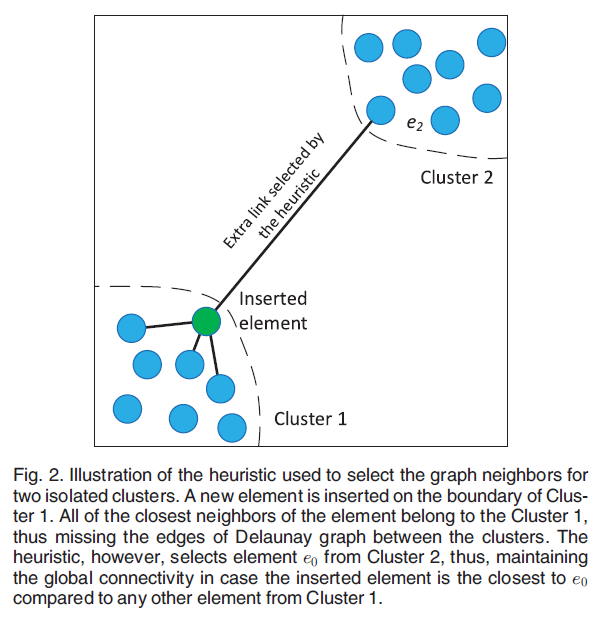
\includegraphics[width=0.5\linewidth]{imgs/hnsw_heuristic.png}
    \end{figure}
\end{frame}

\begin{frame}{HNSW - Comparação}
    \begin{figure}
        \centering
        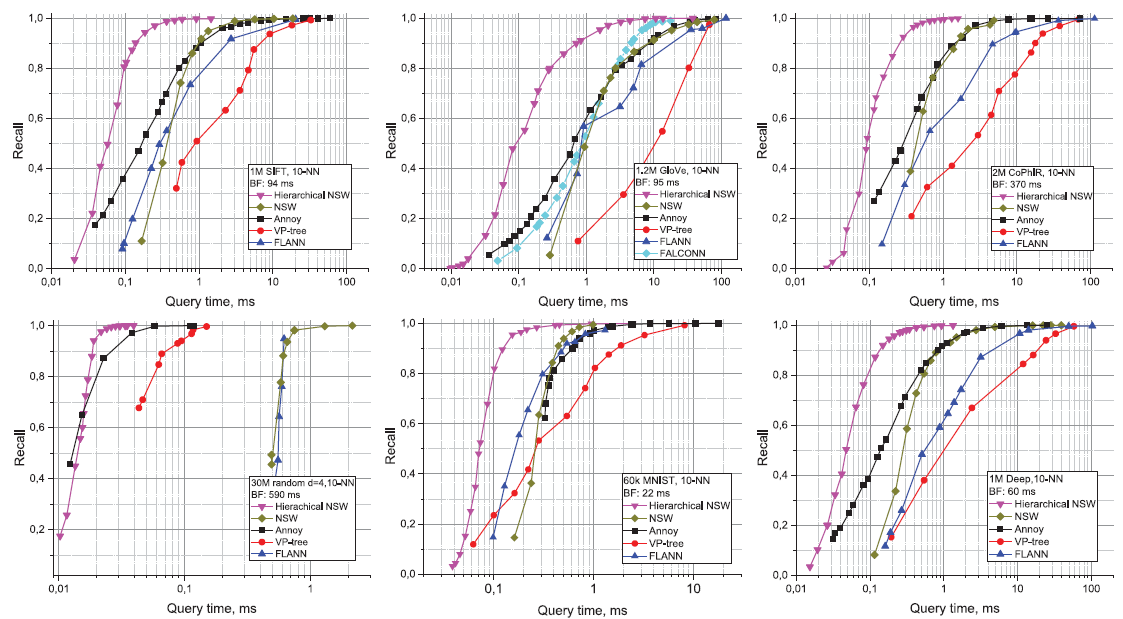
\includegraphics[width=0.85\linewidth]{imgs/hnsw_results.png}
        \caption{\scriptsize BF significa o tempo do força bruta. Para cima e esquerda é melhor.}
    \end{figure}
\end{frame}

\begin{frame}{Em progresso...}
    \begin{itemize}
        \item Cada vértice no grafo, pode ser uma estrutura mais complexa do que um vetor. O cálculo de distância pode ser uma semimétrica.
        \item Limitações com relação ao uso de memória.
        \item Implementações: HNSWLIB (do autor), Faiss (Meta), Milvus.
    \end{itemize}
\end{frame}

\end{document}
